\section{Ablation Study} \label{sec:ablation}
% \subsection{Impact of the Sampling Hyperparameter \(\alpha\)}

To understand the influence of our sampling strategies, we conducted an ablation study on the hyperparameter \(\alpha\), which controls the degree of class balancing in our samplers. The parameter \(\alpha\) interpolates between the original data distribution (\(\alpha=0\)) and a perfectly uniform class distribution (\(\alpha=1\)). A higher value of \(\alpha\) enforces more aggressive rebalancing by increasing the sampling rate of minority classes. The results of this analysis across three datasets are presented in Table~\ref{tab:merged_comparison}. 

On CIFAR-10, a higher degree of balancing generally proves beneficial when using the advanced \textbf{I}mbalanced \textbf{L}ight\textbf{W}eight \textbf{H}ybrid (ILWH) training scheme. For WRBS, performance peaks at \(\alpha=1.0\) (82.41\%), while for WFBS, the sweet spot is at \(\alpha=0.7\) (82.20\%). This indicates that for this 10-class problem, aggressively rebalancing the dataset allows the model to better learn minority class features without significantly degrading performance on majority classes.

In contrast, on the more complex CIFAR-100 dataset, a less aggressive balancing strategy (\(\alpha=0.5\)) consistently yields the best results for both WRBS (47.82\%) and WFBS (45.79\%) under the ILWH setting. Performance for both samplers degrades as \(\alpha\) increases toward 1.0. This suggests that in a fine-grained classification scenario with many classes, overly aggressive sampling of the rare classes can cause the model to under-learn the diverse features present in the more populated ``head'' classes, ultimately harming overall accuracy.

The results on SVHN-10 present another interesting case. Here, the standard \textbf{Random} sampling, when paired with ILWH, achieves the highest accuracy (85.19\%), outperforming all tuned \(\alpha\) values for both WRBS and WFBS. This suggests that for certain datasets, the powerful regularization provided by the training method ILWH may be more impactful than the specific batch-level balancing strategy, making aggressive re-sampling less critical or even slightly detrimental.

In conclusion, the choice of \(\alpha\) is not one-size-fits-all. While stronger balancing can be effective, it carries the risk of model underfitting on majority classes. Our results suggest using a conservative value like \(\alpha=0.5\) as a strong starting point, especially for complex datasets with many classes, and treating it as a key hyperparameter to be tuned based on the specific characteristics of the task at hand.
% \paragraph{AutoAugment}
% AutoAugment introduces a learned sequence of augmentation policies, which diversifies the training data by applying a complex set of transformations discovered through a search process. During training, the exposure of the network to such a wide array of augmented samples aims to enhance model robustness by preventing it from overfitting to the original, potentially limited, training instances. The subsequent normalization of these augmented images, based on the dataset's statistical properties, is anticipated to stabilize the training trajectory and potentially accelerate convergence by standardizing the input distribution presented to the network. The core impact on training is the broadened feature space exploration, compelling the model to learn more generalizable representations.

% \paragraph{RandAugment}
% RandAugment simplifies the automated augmentation paradigm by applying a randomly selected sequence of $N$ transformations, each with a global magnitude $M$. This approach introduces a controlled yet stochastic element to the training data pipeline. The random application of these transformations acts as a dynamic regularizer, potentially smoothing the loss landscape and guiding the model towards flatter minima, which are often associated with better generalization. By varying $N$ and $M$, the intensity of augmentation can be tuned, directly influencing the degree of perturbation in the training samples and thereby affecting the model's sensitivity to input variations learned during training. The primary effect on training is the consistent introduction of novel data variations with minimal computational overhead compared to more complex search-based methods.

% \paragraph{Cutout}
% Cutout operates by randomly excising square regions from input images during training. This technique imposes a unique form of spatial regularization, compelling the network to learn from a more comprehensive set of contextual cues within an image, rather than focusing on a few dominant, localized features. By simulating occlusions, Cutout encourages the model to develop more robust and distributed feature representations during the training phase. This can be particularly beneficial in preventing the model from becoming overly reliant on specific visual patterns that might be prevalent in the majority classes or distinctive but not generalizable features of minority classes. Its application during data loading introduces minimal computational burden, making it an efficient method to enhance feature learning throughout the training epochs.



% \section{Potential Lightweight Approaches in Imbalanced Classification}

% The ablation study systematically evaluates the incremental contributions of each component within the proposed lightweight augmentation and sampling pipeline. By sequentially adding components and carefully analyzing their impacts, we uncover the effectiveness, limitations, and interplay among various methods designed to handle imbalanced data learning tasks.

% \paragraph{Impact of Lightweight Data Augmentation}
% To quantify the benefits of lightweight data augmentation methods, we evaluate three widely-used augmentation techniques: Cutout, AutoAugment, and RandAugment. Applying Cutout—randomly masking regions of input images—provides modest improvement by forcing the model to consider broader contextual features. However, this technique sometimes inadvertently masks critical features for minority classes, thus reducing its potential impact in scenarios with severe class imbalance. Subsequently, AutoAugment, which leverages reinforcement learning to automatically determine optimal augmentation policies, shows notable improvement. Its strength lies in its adaptability, discovering augmentation strategies suited specifically for the CIFAR-10 dataset. However, AutoAugment incurs considerable computational costs due to its policy search phase, limiting practical deployment, especially in resource-constrained environments. RandAugment simplifies this search by applying randomly selected transformations with adjustable intensity parameters. Our results indicate RandAugment consistently achieves superior or comparable performance compared to AutoAugment, but with significantly reduced computational overhead. This highlights RandAugment as a particularly suitable choice when balancing computational efficiency and performance improvements.

% % To further strengthen the insights provided here, an additional experiment evaluating computational resource usage (e.g., training time and memory consumption) explicitly comparing RandAugment and AutoAugment would be beneficial. A graphical illustration highlighting computational cost versus performance gains would provide valuable empirical evidence for recommending RandAugment in practice.

% \paragraph{Integration of Mixup and DRW}
% The integration of Mixup augmentation with Deferred Re-weighting (DRW) significantly enhances model performance. Mixup interpolates between pairs of training samples, thereby softening decision boundaries and improving generalization across imbalanced classes. DRW dynamically adjusts class weights during training, ensuring minority classes receive appropriate emphasis as training progresses. Our results confirm that combining Mixup with DRW consistently improves classification accuracy across all sampling strategies evaluated. Nonetheless, the performance depends heavily on careful tuning of Mixup parameters (such as the mixing parameter $\alpha$). Incorrect parameterization may introduce excessive noise, especially in minority classes, negatively affecting model generalization. To strengthen this finding, conducting experiments analyzing the sensitivity of model performance to the Mixup hyperparameter $\alpha$ would provide valuable insights. Visualization of model accuracy and loss curves as a function of $\alpha$ would clearly illustrate optimal operational ranges, enhancing both theoretical insights and practical guidelines.

% \paragraph{Analysis of Sampling Strategies}
% Next, we assess two sampling techniques: WeightedRandomBatchSampler (WRBS) and WeightedFixedBatchSampler (WFBS). WRBS dynamically samples data based on class-specific weights, ensuring diverse class representations within each batch. Experimental results confirm WRBS effectively improves minority class accuracy by providing richer exposure to underrepresented samples during training. However, WRBS-induced variability in batch compositions across epochs may cause fluctuations in training stability and potentially affect convergence. Conversely, WFBS enforces strict, fixed class proportions per batch, ensuring stable and consistent batch compositions. While WFBS generally improves minority-class generalization due to consistency, its rigid structure makes it less adaptable to datasets with evolving distributions. Consequently, WFBS may limit performance improvements when class distributions dynamically shift during training or across datasets. A comparative analysis between these two sampling methods using additional datasets with differing class-imbalance characteristics would substantially enhance generalization of these findings. Additionally, visualizations of training dynamics (such as accuracy, precision, and loss convergence graphs) under WRBS versus WFBS would clarify their respective strengths and weaknesses, assisting practitioners in selecting the optimal sampling method for their specific use-case.

% \paragraph{DRW}

\begin{figure}[htb]
    \centering
    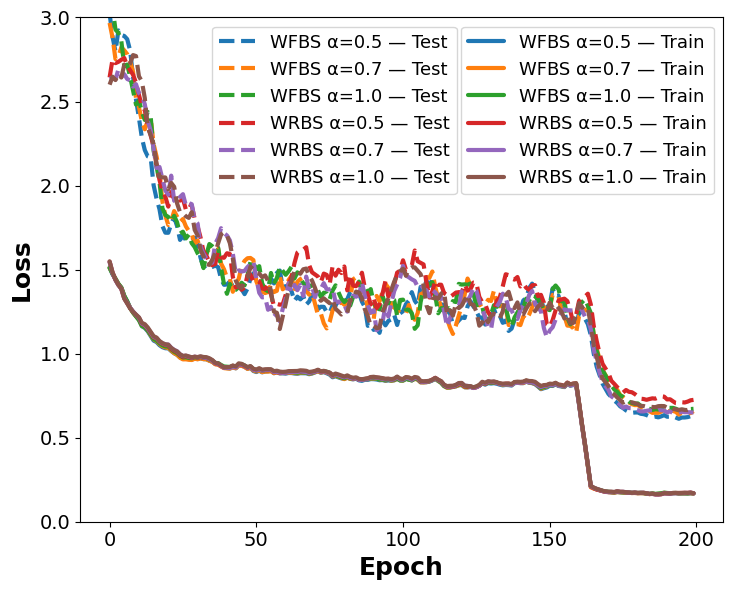
\includegraphics[width=0.9\columnwidth]{drw_affect.png}
        \caption{Effect of applying DRW. After the $160^{th}$ epoch, we apply DRW and observe that the losses have significantly decreased.}
\label{fig:drw_affect}
\end{figure}
\begin{figure}[htb]
    \centering
    \begin{subfigure}[b]{0.48\columnwidth}
        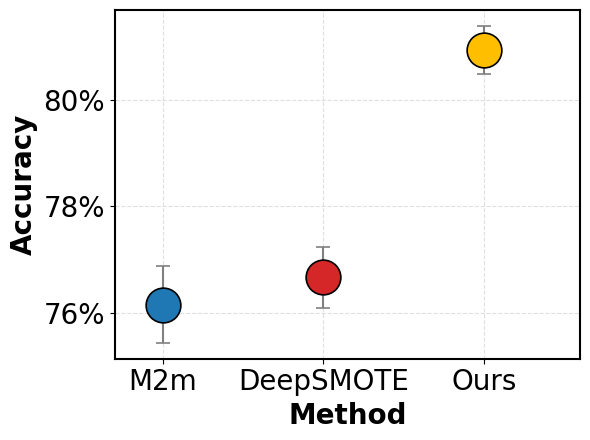
\includegraphics[width=\columnwidth]{cifar10_comparision.png}
        \caption{CIFAR-10}
        % \vspace{-7pt}
        \label{fig:cifar10_comparisionA}
    \end{subfigure}
    \begin{subfigure}[b]{0.48\columnwidth}
        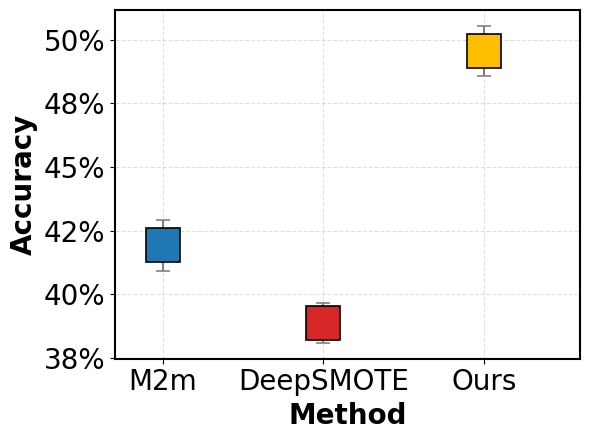
\includegraphics[width=\columnwidth]{cifar100_comparision.png}
        \caption{CIFAR-100}
        % \vspace{-7pt}
        \label{fig:cifar100_comparisionB}
    \end{subfigure}
    \caption{The comparison of our lightweight method and the other resource-intensive methods model performance on CIFAR-10 and CIFAR-100 dataset. This result (M2m, DeepSMOTE \cite{cheng2023smote} and Ours)  demonstrates that our method archive competitive performance.}   \label{fig:comparision_m2m_deepSMOTE_Ours}
\end{figure}
\begin{figure}
    \centering
    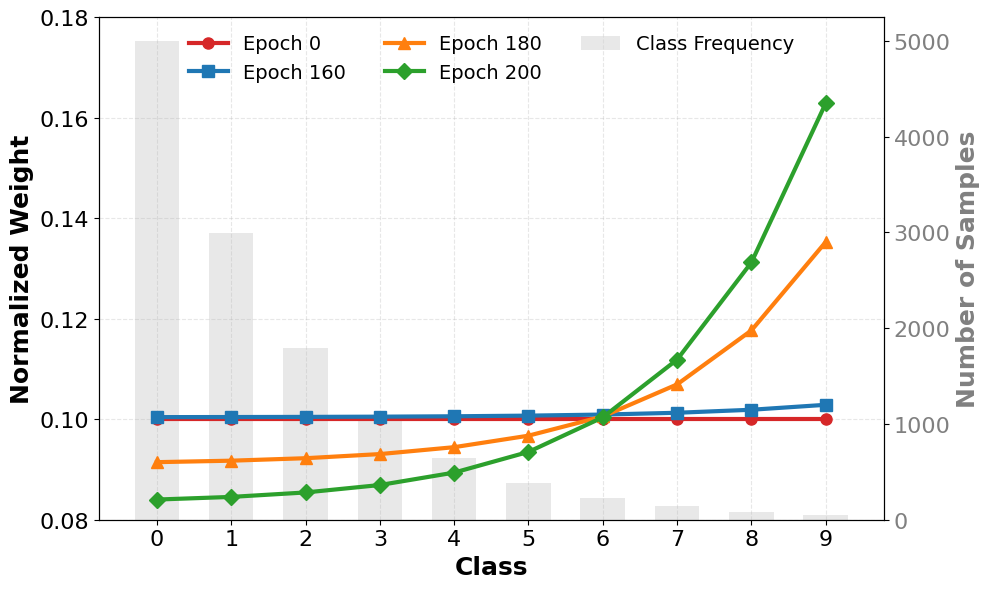
\includegraphics[width=\columnwidth]{weight_dist.png}
        % \vspace{-7pt}
    \caption{Weight distribution for CIFAR-10 classes before and after applying DRW.}
    \label{fig:weight_dist}
\end{figure}

% \begin{table*}[t]
% \centering
% \caption{Performance comparison of different sampling methods and augmentations across CIFAR-10, SVHN-10, and CINIC-10 datasets. \label{tab:drw_results_cifar_svhn_cinic}}
% \scalebox{0.68}{
% \begin{tabular}{l|c| cccc | cccc | cccc }
% \toprule
% \toprule
% \multirow{2}{*}{Sampling} & \multirow{2}{*}{Augmentation} 
%     & \multicolumn{4}{c}{\textbf{CIFAR-10}} 
%     & \multicolumn{4}{c}{\textbf{SVHN-10}} 
%     & \multicolumn{4}{c}{\textbf{CINIC-10}} \\
% \cmidrule(lr){3-6} \cmidrule(lr){7-10} \cmidrule(lr){11-14}
% & & ERM & DRW & Mixup & ILWH (Ours) 
%   & ERM & DRW & Mixup & ILWH (Ours) 
%   & ERM & DRW & Mixup & ILWH (Ours) \\
% \midrule
% \midrule
% \multirow{4}{*}{\textbf{Random}} 
%     & Baseline & 72.74\scriptsize{$\pm$0.42} & 76.03\scriptsize{$\pm$0.05} &   73.37\scriptsize{$\pm$0.15} & \textbf{82.19\scriptsize{$\pm$0.17}} 
%                 & 81.60$\pm$0.28 & 80.57$\pm$0.79 & 80.73$\pm$0.43 & 85.52$\pm$0.26 
%                 & 60.65$\pm$0.39 & 64.29$\pm$0.22 &  63.75$\pm$0.57 & 71.21$\pm$0.19 \\
%     % \cmidrule(lr){2-14}
%     & Cutout   & 72.15$\pm$0.48 & 75.65$\pm$0.39 & 73.32$\pm$0.66 & 81.84$\pm$0.12 
%                 & 85.40$\pm$0.63 & 86.78$\pm$0.30 &  81.53$\pm$0.78  & 86.32$\pm$0.11 
%                 & 64.52$\pm$0.42  & 68.55$\pm$0.32 &  65.70$\pm$0.68 & 73.55$\pm$0.16 \\
%     % \cmidrule(lr){2-14}
%     & AutoAug  & 75.15 $\pm$ 0.35 & 79.08 $\pm$ 0.46 & 72.96 $\pm$ 0.21   & 81.97 $\pm$ 0.13 
%                 & \textbf{85.78 $\pm$ 0.30} & \textbf{86.80 $\pm$ 0.83} & 85.86 $\pm$ 0.21   & \textbf{88.20 $\pm$ 0.49} 
%                 & 63.83 $\pm$ 0.20 & 68.99 $\pm$ 0.50 &  65.35  $\pm$ 0.32    & 73.36 $\pm$ 0.29  \\
%     % \cmidrule(lr){2-14}
%     & RandAug  & \textbf{75.72 $\pm$ 0.38} & \textbf{80.94 $\pm$ 0.12} &   73.77 $\pm$ 0.26 & 81.36 $\pm$ 0.61 
%                 & 84.62 $\pm$ 0.43 & 85.58 $\pm$ 0.91 &  83.08 $\pm$ 0.65   & 86.82 $\pm$ 0.33 
%                 & 64.71 $\pm$ 0.06 & 70.52 $\pm$ 0.27  &  65.92 $\pm$ 0.46  & 73.61 $\pm$  0.16 \\
% \midrule
% \multirow{4}{*}{\textbf{WRBS}} 
%     & Baseline & -- & -- & -- & -- & -- & -- & -- & -- & 60.68 $\pm$ 0.45 & -- & -- & -- \\
%     % \cmidrule(lr){2-14}
%     & Cutout   & -- & -- & -- & -- & -- & -- & -- & -- &  64.34 $\pm$ 0.45  & -- & -- & -- \\
%     % \cmidrule(lr){2-14}
%     & AutoAug  & -- & -- & -- & -- & -- & -- & -- & -- & 63.81 $\pm$ 0.51  & -- & -- & -- \\
%     % \cmidrule(lr){2-14}
%     & RandAug  & -- & -- & -- & -- & -- & -- & -- & -- & 65.16 $\pm$ 0.36 & -- & -- & -- \\
% \midrule
% \multirow{4}{*}{\textbf{WFBS}} 
%     & Baseline & 71.80 $\pm$ 0.60&   75.21 $\pm$ 0.65    &   73.36 $\pm$ 0.39  &  81.91  $\pm$ 0.33   & 80.41 $\pm$ 0.20 &   80.43 $\pm$ 0.83 &  81.14 $\pm$ 0.29  & 85.59 $\pm$ 0.44 & --  & -- & -- & -- \\
%     % \cmidrule(lr){2-14}
%     & Cutout   &  75.38 $\pm$ 0.46 & 79.90 $\pm$  0.79 &   73.49 $\pm$ 0.65 &   81.47 $\pm$ 0.17 & 84.01 $\pm$ 0.50 &   85.64 $\pm$ 1.04 &  82.49 $\pm$ 1.28 &  86.14 $\pm$ 0.59 &   -- &  --  & -- & -- \\
%     % \cmidrule(lr){2-14}
%     & AutoAug  & 74.23 $\pm$ 0.30 & 79.54 $\pm$  0.52 &  73.63 $\pm$ 0.86   & 82.00 $\pm$ 0.17  & 85.30 $\pm$  0.70 &  86.39 $\pm$ 0.64   &  85.05 $\pm$ 0.31 & 88.43 $\pm$ 0.56 & --  & -- & -- & -- \\
%     % \cmidrule(lr){2-14}
%     & RandAug  &  75.24 $\pm$  1.20  &  80.92 $\pm$ 0.24  &  74.03 $\pm$ 0.41 &  81.60 $\pm$ 0.21  & 83.92 $\pm$  1.71 &   84.85  $\pm$ 0.94 &   83.29 $\pm$ 0.78  &  87.46 $\pm$  0.41  & --  & -- & -- & -- \\
% \bottomrule
% \bottomrule
% \end{tabular}}
% \end{table*}

% In your preamble
% \newcommand{\valpm}[2]{#1{\tiny $\pm$#2}}
\begin{table*}[htb]
\centering
\caption{Performance comparison of different sampling methods and augmentations across CIFAR-10, SVHN-10, and CINIC-10 datasets with imbalance ratio 0.01. Best results are highlighted in \textbf{bold} while the runner up is \underline{\textit{underlined}}.}.
\label{tab:drw_results_cifar_svhn_cinic}
\renewcommand{\arraystretch}{1.5}
\setlength{\tabcolsep}{1.0pt}
\scalebox{0.80}{
\begin{tabular}{lc cccc cccc cccc }
\toprule
\toprule
\multirow{2}{*}{Sampling} & \multirow{2}{*}{Augmentation} 
    & \multicolumn{4}{c}{\textbf{CIFAR-10}} 
    & \multicolumn{4}{c}{\textbf{SVHN-10}} 
    & \multicolumn{4}{c}{\textbf{CINIC-10}} \\
\cmidrule(lr){3-6} \cmidrule(lr){7-10} \cmidrule(lr){11-14}
& & ERM & DRW & Mixup & ILWH (Ours) 
  & ERM & DRW & Mixup & ILWH (Ours) 
  & ERM & DRW & Mixup & ILWH (Ours) \\
\midrule
\midrule
\multirow{4}{*}{\textbf{Random}} 
    & Baseline & \valpm{72.74}{0.42} & \underline{\valpm{76.03}{0.05}} & \valpm{73.37}{0.15} & \textbf{\valpm{82.19}{0.17}} 
                & \underline{\valpm{81.60}{0.28}} & \valpm{80.57}{0.79} & \valpm{80.73}{0.43} & \textbf{\valpm{85.52}{0.26}} 
                & \valpm{60.65}{0.39} & \underline{\valpm{64.29}{0.22}} & \valpm{63.75}{0.57} & \textbf{\valpm{71.21}{0.19}} \\
    & Cutout   & \valpm{72.15}{0.48} & \underline{\valpm{75.65}{0.39}} & \valpm{73.32}{0.66} & \textbf{\valpm{81.84}{0.12}} 
                & \valpm{85.40}{0.63} & \textbf{\valpm{86.78}{0.30}} & \valpm{81.53}{0.78} & \underline{\valpm{86.32}{0.11}} 
                & \valpm{64.52}{0.42} & \underline{\valpm{68.55}{0.32}} & \valpm{65.70}{0.68} & \textbf{\valpm{73.55}{0.16}} \\
    & AutoAug  & \underline{\valpm{79.08}{0.46}} & \valpm{75.15}{0.35} & \valpm{72.96}{0.21} & \textbf{\valpm{81.97}{0.13}} 
                & \valpm{85.78}{0.30} & \underline{\valpm{86.80}{0.83}} & \valpm{85.86}{0.21} & \textbf{\valpm{88.20}{0.49}} 
                & \valpm{63.83}{0.20} & \underline{\valpm{68.99}{0.50}} & \valpm{65.35}{0.32} & \textbf{\valpm{73.36}{0.29}} \\
    & RandAug  & \underline{\valpm{80.94}{0.12}} & \valpm{75.72}{0.38} & \valpm{73.77}{0.26} & \textbf{\valpm{81.36}{0.61}} 
                & \valpm{84.62}{0.43} & \underline{\valpm{85.58}{0.91}} & \valpm{83.08}{0.65} & \textbf{\valpm{86.82}{0.33}} 
                & \valpm{64.71}{0.06} & \underline{\valpm{70.52}{0.27}} & \valpm{65.92}{0.46} & \textbf{\valpm{73.61}{0.16}} \\
\midrule
\multirow{4}{*}{\textbf{WRBS}} 
    & Baseline &  \valpm{71.14}{0.22} & \underline{\valpm{75.32}{0.42}} & \valpm{74.65}{0.10} & \textbf{\valpm{82.01}{0.46}} 
                & \underline{\valpm{82.96}{0.85}} & \valpm{81.07}{1.60} & \valpm{81.39}{0.62} & \textbf{\valpm{84.60}{2.02}} 
                & \valpm{60.68}{0.45} & \valpm{58.02}{1.80} & \underline{\valpm{62.42}{0.34}} & \textbf{\valpm{68.32}{0.17}} \\
    & Cutout   & \valpm{71.65}{1.21} & \underline{\valpm{75.46}{0.61}} & \valpm{73.46}{0.82} & \textbf{\valpm{81.30}{0.37}} 
                & \valpm{81.98}{1.43} & \underline{\valpm{84.49}{1.95}} & \valpm{83.20}{0.47} & \textbf{\valpm{85.33}{1.34}} 
                & \valpm{64.34}{0.45} & \valpm{61.74}{0.75} & \underline{\valpm{64.96}{0.74}} & \textbf{\valpm{69.07}{0.23}} \\
    & AutoAug  & \valpm{71.64}{0.06} & \underline{\valpm{75.31}{0.41}} & \valpm{73.77}{0.40} & \textbf{\valpm{82.35}{0.25}} 
                & \valpm{85.30}{0.70} & \underline{\valpm{86.39}{0.64}} & \valpm{86.07}{2.31} & \textbf{\valpm{88.43}{0.56}} 
                & \valpm{63.81}{0.51} & \valpm{61.48}{0.63} & \underline{\valpm{64.57}{0.42}} & \textbf{\valpm{69.61}{0.12}} \\
    & RandAug  & \valpm{71.52}{0.32} & \underline{\valpm{75.27}{0.21}} & \valpm{73.39}{0.11} & \textbf{\valpm{82.10}{0.44}} 
                & \valpm{85.17}{2.19} & \textbf{\valpm{87.45}{0.24}} & \valpm{87.35}{0.30} & \underline{\valpm{87.44}{0.42}} 
                & \valpm{65.16}{0.36} & \underline{\valpm{66.67}{0.38}} & \valpm{65.66}{0.35} & \textbf{\valpm{72.18}{0.39}} \\
\midrule
\multirow{4}{*}{\textbf{WFBS}} 
    & Baseline & \valpm{71.80}{0.60} & \underline{\valpm{75.21}{0.65}} & \valpm{73.36}{0.39} & \textbf{\valpm{81.91}{0.33}} 
                & \valpm{80.41}{0.20} & \valpm{80.43}{0.83} & \underline{\valpm{81.14}{0.29}} & \textbf{\valpm{85.59}{0.44}} 
                & \valpm{56.32}{0.90} & \valpm{60.62}{0.17} & \underline{\valpm{61.98}{0.27}} & \textbf{\valpm{69.43}{0.36}} \\
    & Cutout   & \underline{\valpm{79.90}{0.79}} & \valpm{75.38}{0.46} & \valpm{73.49}{0.65} & \textbf{\valpm{81.47}{0.17}} 
                & \valpm{84.01}{0.50} & \underline{\valpm{85.64}{1.04}} & \valpm{82.49}{1.28} & \textbf{\valpm{86.14}{0.59}} 
                & \valpm{56.74}{0.67} & \valpm{62.91}{0.35} & \underline{\valpm{63.31}{0.14}} & \textbf{\valpm{70.81}{0.21}} \\
    & AutoAug  & \underline{\valpm{79.54}{0.52}} & \valpm{74.23}{0.30} & \valpm{73.63}{0.86} & \textbf{\valpm{82.00}{0.17}} 
                & \valpm{85.30}{0.70} & \underline{\valpm{86.39}{0.64}} & \valpm{85.05}{0.31} & \textbf{\valpm{88.43}{0.56}} 
                & \valpm{61.47}{0.45} & \underline{\valpm{66.32}{0.12}} & \valpm{61.11}{0.28} & \textbf{\valpm{71.86}{0.16}} \\
    & RandAug  & \underline{\valpm{80.92}{0.24}} & \valpm{75.24}{1.20} & \valpm{74.03}{0.41} & \textbf{\valpm{81.60}{0.21}} 
                & \underline{\valpm{84.85}{0.94}} & \valpm{83.92}{1.71} & \valpm{83.29}{0.78} & \textbf{\valpm{87.46}{0.41}} 
                & \valpm{62.85}{0.55} & \underline{\valpm{66.31}{0.36}} & \valpm{66.02}{0.04} & \textbf{\valpm{71.68}{0.16}} \\
\bottomrule
\bottomrule
\end{tabular}}
\end{table*}
\begin{table*}[htb]
\centering
\caption{Performance comparison of different sampling methods and augmentations across CIFAR-100 and TinyImageNet-200 (TINY-200) datasets with imbalance ratio 0.01. Best results are highlighted in \textbf{bold} while the runner up is \underline{\textit{underlined}}.}
\label{tab:drw_results_cifar100_tiny}
\renewcommand{\arraystretch}{1.5}
\setlength{\tabcolsep}{3pt}
\scalebox{0.99}{
\begin{tabular}{lc cccc  cccc }
\toprule
\toprule
\multirow{2}{*}{Sampling} & \multirow{2}{*}{Augmentation} 
    & \multicolumn{4}{c}{\textbf{CIFAR-100}} 
    & \multicolumn{4}{c}{\textbf{TINY-200}} \\
\cmidrule(lr){3-6} \cmidrule(lr){7-10}
& & ERM & DRW & Mixup & ILWH (Ours) 
  & ERM & DRW & Mixup & ILWH (Ours) \\
\midrule
\midrule
\multirow{4}{*}{\textbf{Random}} 
    & Baseline & \valpm{38.87}{0.71} & \valpm{39.46}{0.50} & \underline{\valpm{41.57}{0.46}} & \textbf{\valpm{47.07}{0.47}} 
                & \underline{\valpm{34.17}{0.37}} & \valpm{33.90}{0.41} & \valpm{33.69}{0.29} & \textbf{\valpm{38.69}{0.10}} \\
    & Cutout   & \valpm{43.37}{0.05} & \underline{\valpm{46.12}{0.19}} & \valpm{42.02}{0.59} & \textbf{\valpm{49.56}{0.42}} 
                & \valpm{32.83}{0.36} & \valpm{31.64}{0.36} & \underline{\valpm{34.36}{0.24}} & \textbf{\valpm{39.51}{0.14}} \\
    & AutoAug  & \valpm{42.67}{1.12} & \underline{\valpm{46.48}{0.34}} & \valpm{42.39}{0.34} & \textbf{\valpm{49.53}{0.08}}
                & \valpm{33.95}{0.39} & \valpm{33.62}{0.25} & \underline{\valpm{36.34}{0.19}} & \textbf{\valpm{40.85}{0.47}} \\
    & RandAug  & \valpm{42.19}{0.49} & \underline{\valpm{44.19}{0.32}} & \valpm{42.26}{0.38} & \textbf{\valpm{47.54}{0.34}}
                & \valpm{35.56}{0.44} & \valpm{36.26}{0.26} & \underline{\valpm{36.29}{0.22}} & \textbf{\valpm{39.11}{0.19}} \\
\midrule
\multirow{4}{*}{\textbf{WRBS}} 
    & Baseline & \valpm{39.55}{0.40} & \valpm{40.59}{0.46} & \underline{\valpm{41.01}{0.17}} & \textbf{\valpm{47.17}{0.12}} 
                & \underline{\valpm{32.92}{0.32}} & \valpm{31.87}{0.87} & \valpm{32.68}{0.32} & \textbf{\valpm{33.99}{0.12}} \\
    & Cutout   & \valpm{41.77}{0.45} & \underline{\valpm{44.31}{0.36}} & \valpm{41.71}{0.29} & \textbf{\valpm{47.57}{0.26}} 
                & \underline{\valpm{34.13}{0.05}} & \valpm{30.33}{0.34} & \valpm{32.56}{0.28} & \textbf{\valpm{35.09}{0.31}} \\
    & AutoAug  & \valpm{43.02}{0.21} & \underline{\valpm{46.25}{0.30}} & \valpm{42.21}{0.23} & \textbf{\valpm{49.59}{0.35}}
                & \underline{\valpm{34.23}{0.04}} & \valpm{32.93}{0.16} & \valpm{34.18}{0.13} & \textbf{\valpm{36.73}{0.20}} \\
    & RandAug  & \valpm{43.27}{0.52} & \underline{\valpm{46.65}{0.45}} & \valpm{41.93}{0.14} & \textbf{\valpm{49.29}{0.33}} 
                & \underline{\valpm{35.40}{0.02}} & \valpm{35.10}{0.02} & \valpm{35.13}{0.17} & \textbf{\valpm{38.85}{0.25}} \\
\midrule
\multirow{4}{*}{\textbf{WFBS}} 
    & Baseline & \valpm{37.20}{0.22} & \valpm{38.14}{0.21} & \textbf{\valpm{44.74}{0.61}} & \underline{\valpm{43.16}{0.57}} 
                & \valpm{31.42}{0.23} & \valpm{29.71}{0.57} & \underline{\valpm{32.37}{0.16}} & \textbf{\valpm{34.00}{0.24}} \\
    & Cutout   & \valpm{38.61}{0.44} & \valpm{39.62}{0.19} & \underline{\valpm{43.38}{0.12}} & \textbf{\valpm{43.97}{0.16}} 
                & \valpm{29.49}{0.44} & \valpm{30.34}{0.38} & \underline{\valpm{32.62}{0.07}} & \textbf{\valpm{34.83}{0.18}} \\
    & AutoAug  & \valpm{42.52}{0.45} & \valpm{44.74}{0.61} & \underline{\valpm{45.34}{0.17}} & \textbf{\valpm{49.59}{0.35}} 
                & \valpm{32.53}{0.26} & \valpm{33.45}{0.19} & \underline{\valpm{35.20}{0.08}} & \textbf{\valpm{36.98}{0.27}} \\
    & RandAug  & \valpm{41.73}{0.24} & \valpm{44.26}{0.34} & \underline{\valpm{45.33}{0.11}} & \textbf{\valpm{46.29}{0.54}} 
                & \valpm{33.38}{0.02} & \valpm{33.19}{0.05} & \underline{\valpm{35.26}{0.11}} & \textbf{\valpm{37.57}{0.12}} \\
\bottomrule
\bottomrule
\end{tabular}}
\end{table*}
